\ifdefined\included
\else
\documentclass[english,a4paper,11pt,twoside]{StyleThese}
\usepackage{amsmath,amssymb}             % AMS Math
\usepackage[T1]{fontenc}
\usepackage[utf8x]{inputenc}
\usepackage{babel}
\usepackage{datetime}

\usepackage{lmodern}
\usepackage{tabularx}
%\usepackage{tabular}
\usepackage{multirow}

\usepackage{subfigure}
\usepackage{fancyvrb}
\usepackage{algorithmic}
\usepackage{algorithm}
\usepackage{mathtools}


\usepackage{hhline}
\usepackage[left=1.5in,right=1.3in,top=1.1in,bottom=1.1in,includefoot,includehead,headheight=13.6pt]{geometry}
\renewcommand{\baselinestretch}{1.05}

% Table of contents for each chapter

\usepackage[nottoc, notlof, notlot]{tocbibind}
\usepackage{minitoc}
\setcounter{minitocdepth}{2}
\mtcindent=15pt
% Use \minitoc where to put a table of contents

\usepackage{aecompl}


% Glossary / list of abbreviations

\usepackage[intoc]{nomencl}
\iftoggle{ThesisInEnglish}{%
\renewcommand{\nomname}{Glossary}
}{ %
\renewcommand{\nomname}{Liste des Abréviations}
}

\newcommand{\accom}[1]{\textcolor{red}{[#1]}}

\makenomenclature

% My pdf code

\usepackage{ifpdf}

\ifpdf
  \usepackage[pdftex]{graphicx}
  \DeclareGraphicsExtensions{.jpg}
  \usepackage[a4paper,pagebackref,hyperindex=true]{hyperref}
  \usepackage{tikz}
  \usetikzlibrary{arrows,shapes,calc}
\else
  \usepackage{graphicx}
  \DeclareGraphicsExtensions{.ps,.eps}
  \usepackage[a4paper,dvipdfm,pagebackref,hyperindex=true]{hyperref}
\fi

\graphicspath{{.}{images/}}

%% nicer backref links. NOTE: The flag ThesisInEnglish is used to define the
% language in the back references. Read more about it in These.tex

\iftoggle{ThesisInEnglish}{%
\renewcommand*{\backref}[1]{}
\renewcommand*{\backrefalt}[4]{%
\ifcase #1 %
(Not cited.)%
\or
(Cited in page~#2.)%
\else
(Cited in pages~#2.)%
\fi}
\renewcommand*{\backrefsep}{, }
\renewcommand*{\backreftwosep}{ and~}
\renewcommand*{\backreflastsep}{ and~}
}{%
\renewcommand*{\backref}[1]{}
\renewcommand*{\backrefalt}[4]{%
\ifcase #1 %
(Non cité.)%
\or
(Cité en page~#2.)%
\else
(Cité en pages~#2.)%
\fi}
\renewcommand*{\backrefsep}{, }
\renewcommand*{\backreftwosep}{ et~}
\renewcommand*{\backreflastsep}{ et~}
}

% Links in pdf
\usepackage{color}
\definecolor{linkcol}{rgb}{0,0,0.4} 
\definecolor{citecol}{rgb}{0.5,0,0} 
\definecolor{linkcol}{rgb}{0,0,0} 
\definecolor{citecol}{rgb}{0,0,0}
% Change this to change the informations included in the pdf file

\hypersetup
{
bookmarksopen=true,
pdftitle="Joint Action for Human-Robot Interaction",
pdfauthor="Sandra DEVIN", %auteur du document
pdfsubject="Thesis", %sujet du document
%pdftoolbar=false, %barre d'outils non visible
pdfmenubar=true, %barre de menu visible
pdfhighlight=/O, %effet d'un clic sur un lien hypertexte
colorlinks=true, %couleurs sur les liens hypertextes
pdfpagemode=None, %aucun mode de page
pdfpagelayout=SinglePage, %ouverture en simple page
pdffitwindow=true, %pages ouvertes entierement dans toute la fenetre
linkcolor=linkcol, %couleur des liens hypertextes internes
citecolor=citecol, %couleur des liens pour les citations
urlcolor=linkcol %couleur des liens pour les url
}

% definitions.
% -------------------

\setcounter{secnumdepth}{3}
\setcounter{tocdepth}{2}

% Some useful commands and shortcut for maths:  partial derivative and stuff

\newcommand{\pd}[2]{\frac{\partial #1}{\partial #2}}
\def\abs{\operatorname{abs}}
\def\argmax{\operatornamewithlimits{arg\,max}}
\def\argmin{\operatornamewithlimits{arg\,min}}
\def\diag{\operatorname{Diag}}
\newcommand{\eqRef}[1]{(\ref{#1})}

\usepackage{rotating}                    % Sideways of figures & tables
%\usepackage{bibunits}
%\usepackage[sectionbib]{chapterbib}          % Cross-reference package (Natural BiB)
%\usepackage{natbib}                  % Put References at the end of each chapter
                                         % Do not put 'sectionbib' option here.
                                         % Sectionbib option in 'natbib' will do.
\usepackage{fancyhdr}                    % Fancy Header and Footer

% \usepackage{txfonts}                     % Public Times New Roman text & math font
  
%%% Fancy Header %%%%%%%%%%%%%%%%%%%%%%%%%%%%%%%%%%%%%%%%%%%%%%%%%%%%%%%%%%%%%%%%%%
% Fancy Header Style Options

\pagestyle{fancy}                       % Sets fancy header and footer
\fancyfoot{}                            % Delete current footer settings

%\renewcommand{\chaptermark}[1]{         % Lower Case Chapter marker style
%  \markboth{\chaptername\ \thechapter.\ #1}}{}} %

%\renewcommand{\sectionmark}[1]{         % Lower case Section marker style
%  \markright{\thesection.\ #1}}         %

\fancyhead[LE,RO]{\bfseries\thepage}    % Page number (boldface) in left on even
% pages and right on odd pages
\fancyhead[RE]{\bfseries\nouppercase{\leftmark}}      % Chapter in the right on even pages
\fancyhead[LO]{\bfseries\nouppercase{\rightmark}}     % Section in the left on odd pages

\let\headruleORIG\headrule
\renewcommand{\headrule}{\color{black} \headruleORIG}
\renewcommand{\headrulewidth}{1.0pt}
\usepackage{colortbl}
\arrayrulecolor{black}

\fancypagestyle{plain}{
  \fancyhead{}
  \fancyfoot{}
  \renewcommand{\headrulewidth}{0pt}
}

%\usepackage{MyAlgorithm}
%\usepackage[noend]{MyAlgorithmic}
\usepackage[ED=MITT - STICIA, Ets=INP]{tlsflyleaf}
%%% Clear Header %%%%%%%%%%%%%%%%%%%%%%%%%%%%%%%%%%%%%%%%%%%%%%%%%%%%%%%%%%%%%%%%%%
% Clear Header Style on the Last Empty Odd pages
\makeatletter

\def\cleardoublepage{\clearpage\if@twoside \ifodd\c@page\else%
  \hbox{}%
  \thispagestyle{empty}%              % Empty header styles
  \newpage%
  \if@twocolumn\hbox{}\newpage\fi\fi\fi}

\makeatother
 
%%%%%%%%%%%%%%%%%%%%%%%%%%%%%%%%%%%%%%%%%%%%%%%%%%%%%%%%%%%%%%%%%%%%%%%%%%%%%%% 
% Prints your review date and 'Draft Version' (From Josullvn, CS, CMU)
\newcommand{\reviewtimetoday}[2]{\special{!userdict begin
    /bop-hook{gsave 20 710 translate 45 rotate 0.8 setgray
      /Times-Roman findfont 12 scalefont setfont 0 0   moveto (#1) show
      0 -12 moveto (#2) show grestore}def end}}
% You can turn on or off this option.
% \reviewtimetoday{\today}{Draft Version}
%%%%%%%%%%%%%%%%%%%%%%%%%%%%%%%%%%%%%%%%%%%%%%%%%%%%%%%%%%%%%%%%%%%%%%%%%%%%%%% 

\newenvironment{maxime}[1]
{
\vspace*{0cm}
\hfill
\begin{minipage}{0.5\textwidth}%
%\rule[0.5ex]{\textwidth}{0.1mm}\\%
\hrulefill $\:$ {\bf #1}\\
%\vspace*{-0.25cm}
\it 
}%
{%

\hrulefill
\vspace*{0.5cm}%
\end{minipage}
}

\let\minitocORIG\minitoc
\renewcommand{\minitoc}{\minitocORIG \vspace{1.5em}}

\usepackage{multirow}
%\usepackage{slashbox}

\newenvironment{bulletList}%
{ \begin{list}%
	{$\bullet$}%
	{\setlength{\labelwidth}{25pt}%
	 \setlength{\leftmargin}{30pt}%
	 \setlength{\itemsep}{\parsep}}}%
{ \end{list} }

\newtheorem{definition}{Définition}
\renewcommand{\epsilon}{\varepsilon}

% centered page environment

\newenvironment{vcenterpage}
{\newpage\vspace*{\fill}\thispagestyle{empty}\renewcommand{\headrulewidth}{0pt}}
{\vspace*{\fill}}

\usepackage{tablefootnote}

\sloppy
\begin{document}
\setcounter{chapter}{6} %% Numéro du chapitre précédent ;)
\dominitoc
\faketableofcontents
\fi

\chapter{Combining learning and planning}
\minitoc

\label{ch:Learning}

\section{Motivation}

When it comes to decisional process in robotics, two main schools of though can be distinguished: machine learning and deterministic processes such as planing or states machines. Both ways have their advantages and disadvantages. Learning is usually "cheap" (the decision process is quick) and always proposes a solution to a given problem. However, learning requires either a big amount of data or a long period of learning. Moreover, during the learning period, the robot can produce inconsistent behavior which can be confusing for a potential human collaborator. On the other hand, planing can take into account humans through social rules and ensure the validity of a whole solution. However, planing does not learn from human behavior, and, when it comes to complex tasks or environments, it can become slow to propose a solution. The idea of this work is to propose a solution where we combine planing and learning in the context of human-robot interaction in order to take advantage of both. 

This work has been done in collaboration with ISIR at Paris and more particularly with another PhD student Erwan Renaudo. It has been done in the context of the RoboErgoSum ANR project\footnote{http://roboergosum.isir.upmc.fr/}. This work is based on the work of \cite{renaudo2014design} and has been the subject of a publication in a workshop at the RoMan conference \cite{renaudo2015learning} as well as a part of a journal article \cite{khamassi2016integration}.

\section{Background}

\subsection{Inspiration from neurosciences}

Seminal works on living being behaviors have been done in the late 19th century - beginning of the 20th century - with experiments on mammals. One pioneer work concerning the learning process is the experiment of the cat in a box \cite{thorndike1998animal}. In this experiment, a cat is put in a box each time it is hungry. The cat can see food outside of the box and a system of lever allows it to open the box. Each time the cat is put in the box it takes less time to go out. This experiment allows to show the principle of learning through trial and error. 

Latter, studies have highlighted two main kinds of behavior during decision-making tasks. \textbf{Goal-directed behaviors} are governed by estimates of action-outcome contingencies (i.e. decision-making relies on the prior estimation of the outcome expected after an action or an action sequence) and are mainly active at the beginning of the task. Then, when the animal is well trained in the task under stable conditions, a transfer of control to \textbf{habitual behaviors} governed by stimulus-response associations occurs  \cite{dickinson1985actions}. When rodents, monkeys or humans start a new decision-making task, they appear to initially rely on their goal-directed system. They take time to analyse the structure of the task in order to build an internal model of it, and make slow decisions by planning and inferring the long-term consequences of their possible actions before deciding what to do next. Then as their performance gradually improve, they appear to make quicker and quicker decisions, relying on their habitual system which slowly acquires simple stimulus-response associations to solve the task. Finally, when subjects restart to make errors after a task change, they appear to restart planning within their internal model and thus slow down their decision process before acquiring the new task contingencies \cite{balleine2010human, dolan2013goals}. The coordination of these two learning systems allows mammals to avoid long and costly computations when the environment is sufficiently stable, while still enabling animals to detect environmental changes requiring to update their internal model and replan.

In computational neuroscience models, these behaviors are modeled using the theory of Reinforcement Learning \cite{sutton1998introduction}: model-based and model-free algorithms provide a direct analogy with goal-directed and habitual behaviors \cite{daw2005uncertainty}. More recently, different computational criteria have been proposed to decide when to shift between model-based and model-free experts \cite{pezzulo2013mixed, lesaint2014modelling, viejo2015modeling}. Applied to neuroscience tasks, the work from \cite{daw2005uncertainty} proposes that the most certain expert gets control on the agent, while \cite{keramati2011speed} balance speed and accuracy using the cost of planning versus the gain of information. A third approach proposes, in the context of navigation strategies, that a coordination module learns by reinforcement the most efficient behavior (in terms of average obtained reward) in each state \cite{dolle2010path}.

\subsection{Learning in human-robot interaction}

A major part of robotics decision-making algorithms are based on planning processes which take into account a great number of information (\cite{ingrand2014deliberation}). These approaches to decision-making could be seen as similar to what neuroscientists call the goal-directed system, except that there is most of the time no learning in the system. Such approaches have been extended to HRI by taking into account human-aware costs such as social-rules and humans comfort and preferences \cite{cirillo2010human,Lallement2014hatp}.

Besides, robots learning abilities are still very limited and require the injection of important prior knowledge by the human in the robot’s decision-making system. Early applications of reinforcement learning (RL) algorithms to robotics \cite{hayes1994robot, morimoto2001acquisition, smart2002effective} - some of which being neuro-inspired - produced limited progresses, due to applications to relatively simple problems (with a small number of states and actions), to slowness in learning and to systematic instability observed throughout the learning process. More recent applications of RL to robotics have permitted to deal with more complex and continuous action spaces, enabling to learn efficient sensorimotor primitives \cite{kober2011learning, martins2010learning, stulp2013robot}. These approaches have been extended in HRI to allow robots to learn to collaborate with humans.
In several works, the reward signal is interactively assigned by the human \cite{kaplan2002robotic, knox2012reinforcement} while other works use the human to provide demonstrations to the robot \cite{nicolescu2003natural, thomaz2006reinforcement}.
A method of cross-training is used and compared to standard reinforcement learning algorithms in the context of human-robot teamwork in \cite{nikolaidis2013human}. Cross-training is an interactive planning method in which a human and a robot iteratively switch roles to learn a shared plan for a collaborative task. Such approaches to decision-making could be seen as similar to what neuroscientists call habitual behaviors.

Even if we can find more and more interesting works in HRI concerning planing and learning for the robot to collaborate with humans, there is no work to our knowledge concerning how to combine both approaches into a robotics architecture.

\section{Experts presentation}

Inspired from neuroscience theories and based on the previous work of \cite{renaudo2014design} the aim of this work is to combine goal-directed and habitual behaviors in the context of human-robot Joint Action. To do so, we use two experts which implement these two kinds of behavior. The goal-directed behavior is produced here by HATP (Human-Aware Task Planer), a task planner which has proved its efficiency in the field of human-robot interaction. A Qlearning algorithm allows to implement the habitual behavior. We will describe in this section these two experts and their respective strengths and weakness. The next sections will show how we combined those two experts into two different architectures.

\subsection{HATP}

In our work, the goal-directed behavior is provided by HATP, an HTN (Hierarchical Task Network, \cite{erol1994htn}) task planner which has been conceived to work in the context of human-robot collaboration.  As a HTN planner, HATP uses known preconditions and effects of actions in order to find the best plan that reaches the given goal. It takes as input a list of all possible actions and their description in terms of preconditions and effects and also a description of the current world state as a set of predicates. Then, it looks for the combination of actions that minimizes the solution cost. This cost is computed based on execution time and human-aware costs (e.g the balance of efforts between agents or the waiting time of the human partner). This plan is meant to be executed step by step until the goal is reached. An example of such a plan can be found Fig.~\ref{fig:examplePlan}.

\begin{figure}[!h]
	\centering
    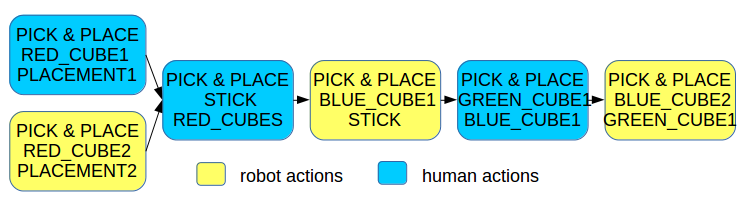
\includegraphics[width=0.9\textwidth]{figs/Chapter7/SharedPlan.png}
    \caption{An example of a Shared Plan computed by HATP. This plan allows a human and a robot to build a stack of colored objects together by placing them one on-top of the others.}
    \label{fig:examplePlan}
\end{figure}

\subsection{Qlearning algorithm (MF)}

The habitual behavior is provided by a model-free reinforcement learning algorithm (MF) that directly learns the state–action associations by caching in each state the earned rewards in the value of each action. In this implementation, the algorithm is implemented as a neural network (see Fig.~\ref{fig:Qlearning}). The network input neurons represent the different possible states and the output neurons encode the estimation of action values in the current state. The weights are modified to associate each state with the most rewarding action in the current task.

A method similar to \cite{brafman2002r} is used to compute the value $Qt(St, a_j)$ of an action $a_j$ in a certain state $S$. $Qt(St, a_j)$ is represented as the scalar product between the input vector and the weights $W_j = (w_{0j} , . . . , w_{Nj})$ linking to this action:
$$Qt(St, a_j) = W_j^t \ . \ (S_t, 1)$$

here we set weights at a positive value to provide an initial optimistic estimate of action values ($w_0$ = 0.5). Weights $W_t$ are updated according to the Qlearning algorithm \cite{watkins1989learning}. The Reward Prediction Error $\delta$ is spread over the weights of the previously active input and the action $a$ done in the corresponding state:
$$\delta = r_t + \gamma_{Hab} \ . \ \underset{b \in A}{max}(W_b^{t-1}) \ . \ S_t - (W_a^{t-1} \ . \ S_{t-1})$$
$$W_a^t = W_a^{t-1} + \alpha_{Hab} \ . \ \delta / \underset{n}{\Sigma}s_{n}$$

with $r_t$ the instant reward received for performing a in $S_{t−1}$ , $\alpha_{Hab}$ the learning rate, $\gamma_{Hab}$ the decay rate of future rewards. The weights are updated locally: only the state from which the action has been performed is updated. Thus, it requires for the agent to visit every known state of the problem to update values.


\begin{figure}[!h]
	\centering
    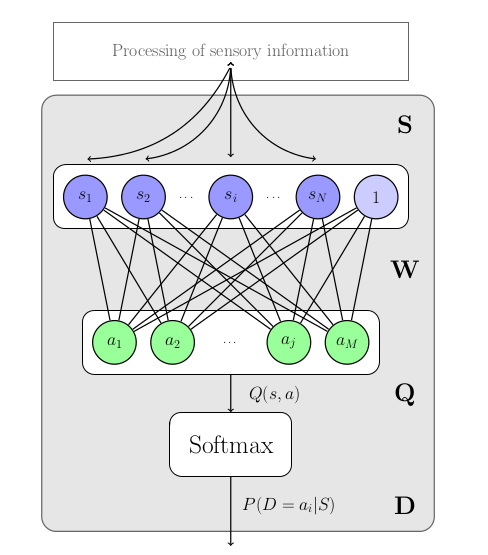
\includegraphics[width=0.6\textwidth]{figs/Chapter7/Qlearning.png}
    \caption{Habitual expert, modeled as a Qlearning algorithm implemented as a neural network. The expert receives a state $S$ which is projected onto the input neurons $s_i$, defining an input activity. This activity is propagated through the network weights $W$ to generate activity of the action layer. This activity corresponds to the values $Q(S, a_j)$, with each neuron coding for a distinct action. This value distribution is converted in probability distribution using a softmax function, which allows the expert to make a decision $D$ on the next action to perform.}
    \label{fig:Qlearning}
\end{figure}

\subsection{Experts comparison}

The two different experts have really different ways to decide of the next action to execute. Both methods have their advantages and disadvantages:
\begin{itemize}
\item HATP looks for a complete solution to achieve the given goal while the MF only looks for the next action which maximize the probability to get a reward. Consequently, HATP ensures the feasibility of the solution proposed but could find itself in a state where it does not find a valid solution and so where it will not be able to propose an action. In the other hand, the MF does not ensure that its proposed action allows to achieve the goal but will always propose an action to perform.
\item As HATP computes a whole plan to achieve the goal, its cost, in the sense of time to take a decision, is far bigger than the one of the MF which only proposes the next action. However, this difference needs to be weighed by the fact that as an HATP plan is composed of several actions, this cost is not needed at each step of the task. Moreover, this cost stay acceptable in a not so complex task.
\item HATP is conceived to produce a robot behavior understandable and acceptable by the human. The actions it proposes will produce a consistent behavior of the robot with which one the human can easily collaborate. For its part, the MF has a long period of learning during which one the behavior produced is inconsistent and can be really disturbing for a human collaborating with the robot. Moreover, each time a change happens in the task, a new learning phase is needed. However, the MF is able to learn to adapt its behavior to the human whereas the HATP policy is defined off-line and can not be updated with the behavior of the human during the interaction.
\end{itemize}


\section{First architecture: a proof of concept}


\subsection{Control architecture}


\begin{figure}[!h]
	\centering
    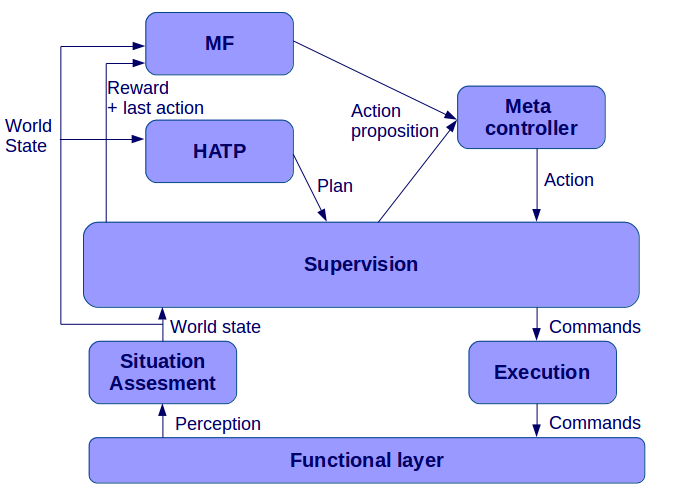
\includegraphics[width=0.8\textwidth]{figs/Chapter7/FirstArchi.png}
    \caption{First tried architecture to combine the two experts. The Situation Assessment module gets data from perception and maintains the current world state. This world state is used by the supervision to compute the reward and by the experts to take decisions. The propositions of the two experts are sent to the meta controller which decides of the action to execute. The supervisor executes the action with the help of lower execution modules.}
    \label{fig:FirstArchi}
\end{figure}

The first architecture we tried to combine the two experts is the one Fig.~\ref{fig:FirstArchi}. In this architecture the two experts are placed in parallel. The execution of a task by the architecture follows several steps:
\begin{itemize}
\item The Situation Assessment module receives data from perception and maintains the world state representation. This world state is represented with predicates (see Sec.~\ref{subsec:taskOne}).
\item The supervisor uses the current world state to compute the reward sent to the MF. This reward is a boolean which is true if the current goal is achieved (see Sec.~\ref{subsec:taskOne}). The supervisor also sends to the MF the last tried action (which was not necessarily the one proposed by the MF) in order to update the learning.
\item The experts decide of the next action to execute based on the current world state. The action proposed by the MF for a given world state is sent directly to the meta controller. Concerning HATP, the supervisor monitors the execution of its plan and sends the next action to execute to the meta controller. A new plan is computed by HATP at the beginning of the task or whenever an unexpected situation happens (an action from the plan fails, the human executes an unexpected action or the robot executes an action proposed by the MF which is not in the current plan).
\item Once the proposition of action from each expert is received, the meta controller decides which action the robot should execute. In this first implementation the meta controller uses a random arbitration: the action is chosen with an equal probability for each expert.
\item The supervisor executes the chosen action with the help of lower execution modules (motion planning, control, ...). 
\end{itemize}
These steps are executed one by one until the goal is achieved.



\subsection{Task}

\label{subsec:taskOne}

This first architecture has been tried in a simple task. Moreover, as the learning part of the architecture requires long learning periods, the tests have been done in simulation.

\begin{figure*}[!h]
\centering
	\subfigure[Initial situation]{
        \centering
        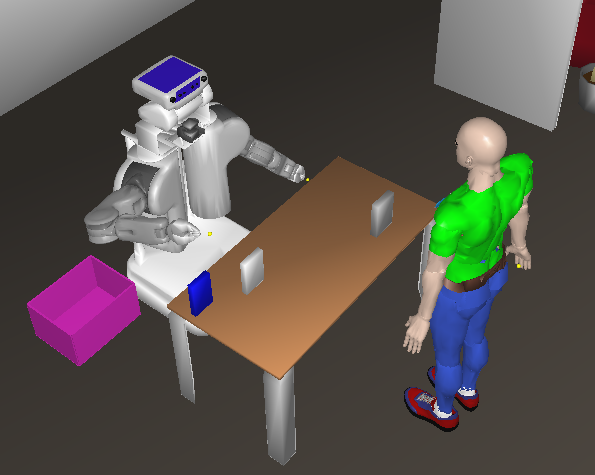
\includegraphics[width=0.45\textwidth]{figs/Chapter7/initFirstTask.png}
       \label{subfig:initFirst}
   }
    %~
	\subfigure[Final situation]{
        \centering
        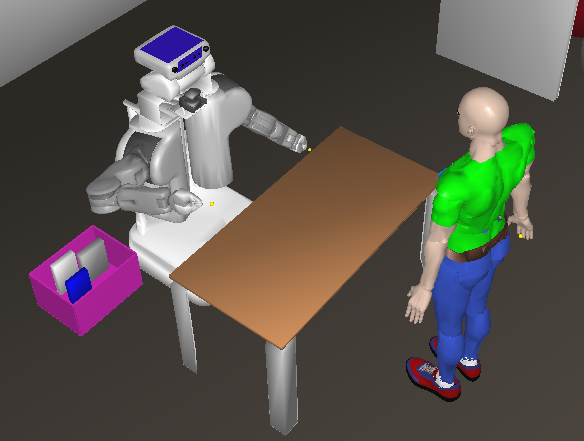
\includegraphics[width=0.47\textwidth]{figs/Chapter7/endFirstTask.png}
       \label{subfig:endFirst}
   }
    \caption{Description of the task used with the first architecture. In this task, the human and the robot have to remove all the objects of the table and put them in the pink box. At the beginning of the interaction two objects are accessible only by the robot and another one only by the human. The box is accessible only by the robot.}
    \label{fig:firstTask}
\end{figure*}

In the chosen task a human and a robot have to "clean a table" together. To do so, they need to remove all the objects from the table and put them in a box (see Fig.~\ref{fig:firstTask}). At the beginning of the interaction two objects are accessible only by the robot and another one only by the human. The box is accessible only by the robot. To achieve the goal, several actions can be executed by the agents:
\begin{itemize}
\item \textbf{Pick an object:} both agents can pick an object accessible by them.
\item \textbf{Throw an object:} the robot can throw an object it has in hand in the box near itself. 
\item \textbf{Give an object:} the robot can give an object to the human.
\item \textbf{Take an object:} the robot can receive an object from the human
\item \textbf{Wait:} the robot can wait for the human to execute an action.
\end{itemize}
All these actions have an impact into the world state. This world state is estimated by the Situation Assessment module and represented with predicates which can be either true or false. For this task, we consider the following predicates:
\begin{itemize}
\item \textbf{<Object, isReachableBy, Agent>:} these predicates represent for each object if it is reachable by the human or the robot.
\item \textbf{<Object, isIn, Box>:} these predicates represent the fact that an object has been thrown in the box.
\item \textbf{<Agent, hasInHand, Object>}: these predicates represent the fact that the human or the robot holds an object.
\end{itemize}
These predicates allow the experts to take their decisions but also the supervisor to compute the reward needed by the MF. The robot will receive a reward whenever all objects are in the box and it performs the \textit{Wait} action. We chose to impose to the robot to perform a \textit{Wait} action at the end of the task in order for it to learn that the task is over and that no more action is needed.

To test our architecture, we compare its performances to the performances of the system running with only the MF and only HATP. We run the experiment in all conditions with a fixed time limit. At the beginning of an experiment the set-up was put at the initial situation (Fig.~\ref{subfig:initFirst}). Once the task is achieved and reward is obtained by the robot, the set-up is put back to the initial situation and the task can be performed again.

As we run the task in simulation, the behavior of the human is also simulated. We chose here to have a collaborative human: it performs all actions HATP planned for him and participates to handover whenever the robot requires one.

\subsection{Results}

\begin{figure*}[!h]
\centering
	\subfigure[Mean cumulative reward on 10 simulations where the robot repeatedly fulfils the task. Errorbars represent the standard deviation from the mean every 100 decisions.]{
        \centering
        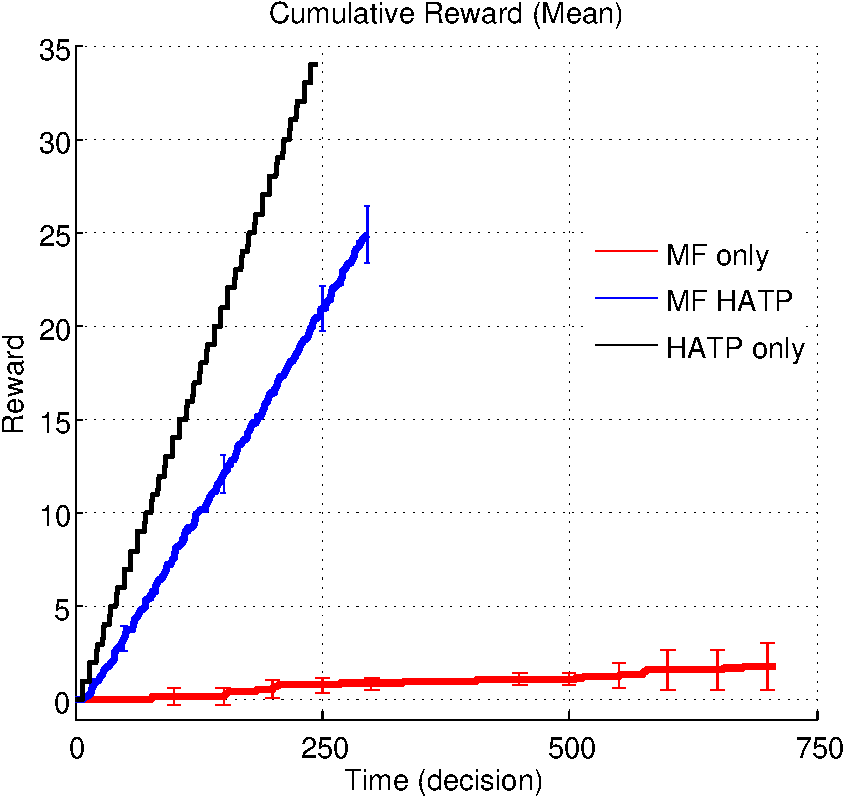
\includegraphics[width=0.45\textwidth]{figs/Chapter7/rewardsFirstTask.pdf}
       \label{subfig:rewardsFirstTask}
   }
    %~
	\subfigure[Number of actions tried per experiment. Dashed line is the mean number of action depending on the control method (MF only, HATP only or combination)]{
        \centering
        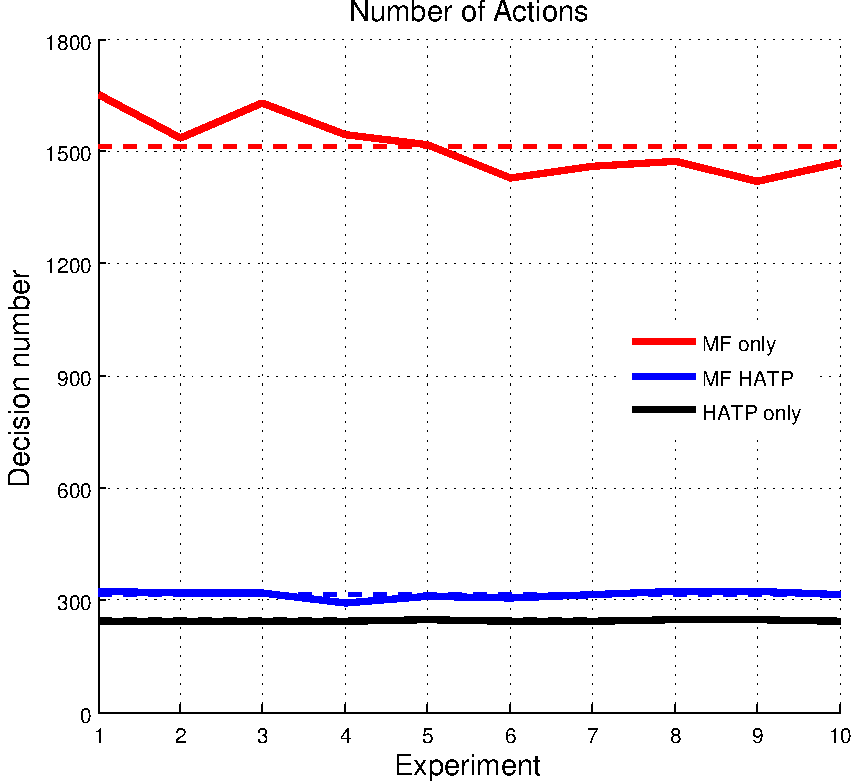
\includegraphics[width=0.45\textwidth]{figs/Chapter7/DecisionNumberFirstTask.pdf}
       \label{subfig:decisionsFirstTask}
   }
    %~
	\subfigure[Mean MF connection weights evolution for MF alone and MF and HATP combination. The amplitude is defined as the sum of the absolute value of weights. Weights are initialized to zero, thus the higher the amplitude is, the more the MF has learnt which action to do.]{
        \centering
        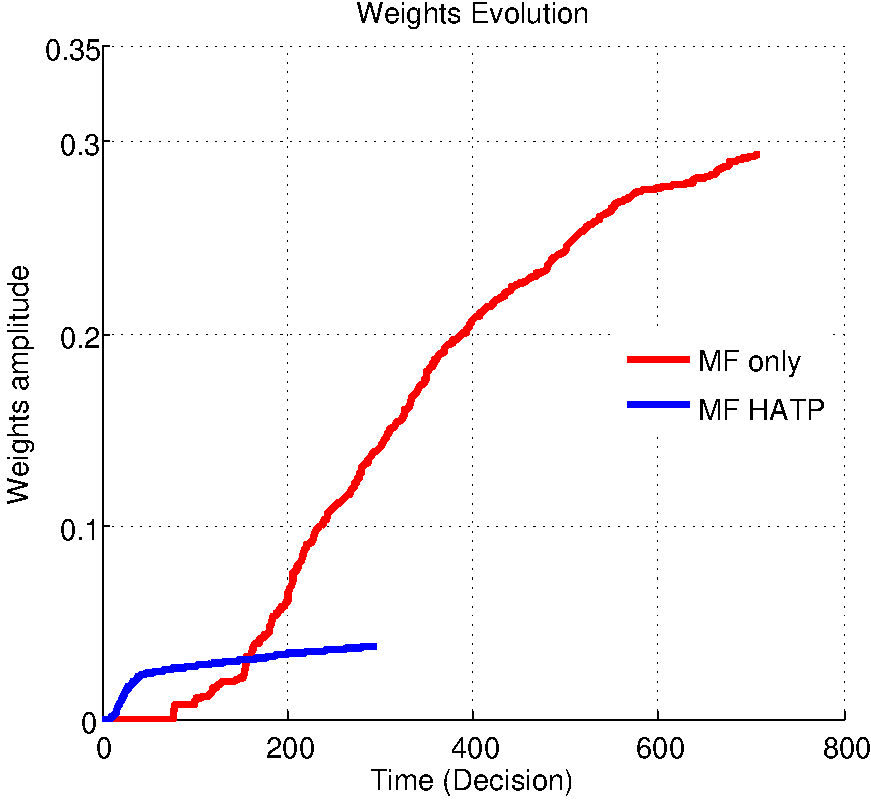
\includegraphics[width=0.45\textwidth]{figs/Chapter7/WeightEvolFirstTask.pdf}
       \label{subfig:weightsFirstTask}
   }
    \caption{Performance of the developed system compared to systems with only the MF and only HATP. The results are for 10 runs of approximately 30 minutes in each condition.}
    \label{fig:resultsFirstTask}
\end{figure*}

The main criteria used to evaluate our system is the cumulative reward obtained in each run (i.e. the number of time the human and the robot manage to achieve the task in a fixed amount of time). We run 10 times the experiment in each condition (MF only, HATP only and the combination of both) for a duration of approximately 30 minutes. The number of rewards obtained are presented in Fig.~\ref{subfig:rewardsFirstTask}. All experiments last the same fixed time, but the number of decisions taken at the end may vary.  We observe a poor performance of the MF alone, which is not able to solve the task more than three times. As the MF has no initial knowledge, it has to discover the right sequence of actions, which is non trivial with the given number of possible states and actions.
The random combination HATP-MF is performing much better than the MF alone, solving the task 25 times in average. However, HATP alone performs even better solving the task 34 times in average. Indeed, the task is easy enough to solve for HATP and the time required to find a plan is negligible here. As the simulated human always performs the actions planned by HATP, the plan found by HATP is always optimal and will never change during the task execution. Accordingly, the random combination of HATP and the MF performs worst as it can include actions proposed by the MF that make the plan non optimal.

Fig.~\ref{subfig:decisionsFirstTask} shows the number of actions proposed to the supervision system during each experiment. We can see that the MF alone suggests twice to three times more actions than HATP or the combination in the same given time. This is mainly due to the way each Expert decides: the MF only needs to compute the values of each action (which is propagating the state activity to action neurons) and to draw an action from the resulting probability distribution. It proposes a lot of unfeasible actions and the supervision system will not spend time to execute them as it will stop to the preconditions verification. HATP checks for action preconditions when planning and so, for each of the action proposed by HATP, the supervisor spend time to execute it (or try to execute it if the action is not really feasible according to the geometry). The number of actions suggested by the combination of Experts is closer to the one with HATP alone while remaining lightly higher. It can be explained by the fact that a part of the actions proposed by the combination comes from HATP and, for the ones coming from the MF, HATP helps it to learn a solution faster, causing it to propose less unfeasible actions.

Finally, we analyze the effect of combination on learning of MF in Fig.~\ref{subfig:weightsFirstTask}. Learning is evaluated by weights amplitude, namely the sum of weights absolute value over actions. The MF starts with weights initialized to zero, each learning step increases or decreases the value of some of the weights, until convergence. The figure shows that learning occurs much earlier for the combination of Experts than when the MF is alone. The combination has a bootstrapping effect and the knowledge about the task from HATP is transferred to the MF. This shows that a human-provided a priori knowledge can be used to guide exploration and learn quicker. Even if not tested in this experiment, this means that a change in task condition for which HATP can find a new plan can be learnt quickly by the MF, so the robot will be able to adapt to the new conditions without taking too much time.

\subsection{Intermediate conclusion}

The first results obtained with this architecture allow to show that the combination of HATP and the MF allows to bootstrap the MF and to learn faster a policy to achieve the goal.

However, this task is too simple for HATP to be in difficulty when deciding alone. The purpose of the second task and architecture presented in the next section is to show the benefits of the combination of the two experts and more particularly how HATP can benefits from the MF. Moreover, we want to test the reaction of our system to changes in the task as well as a more elaborated arbitration criteria for the meta controller.


\section{Second architecture: the limitations}

\subsection{Control architecture}

\begin{figure}[!h]
	\centering
    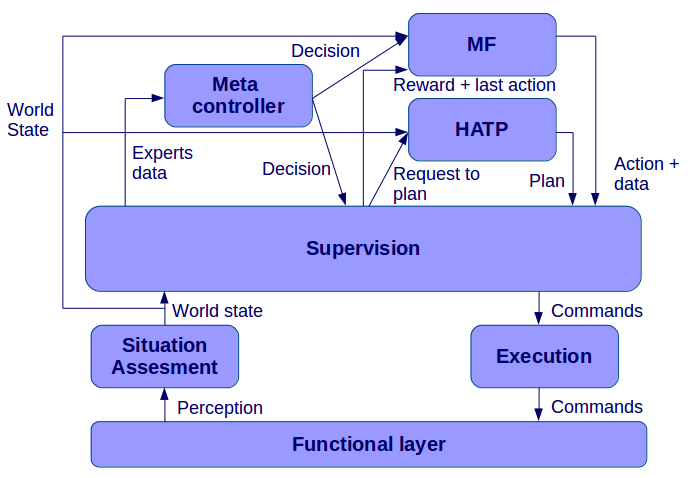
\includegraphics[width=0.8\textwidth]{figs/Chapter7/SecondArchi.png}
    \caption{Second tried architecture to combine the two experts. The Situation Assessment module gets data from perception and maintains the current world state. This world state is used by the supervision to compute the reward and by the experts to take decisions. Here the meta controller is placed upstream from the two experts. It first decides which expert should propose an action. Then, the supervisor executes the action of the chosen expert with the help of lower execution modules.}
    \label{fig:SecondArchi}
\end{figure}

One of the advantage of the MF against HATP is its computation time. In the previous architecture, both experts where consulted before the meta controller took a decision. Consequently, even if the MF was chosen, we still lost time to compute plans with HATP. In order to solve this issue, we modified the previous architecture as shown in Fig.~\ref{fig:SecondArchi}. 

In the new architecture, the meta controller is placed upstream from the two experts. Consequently, the order of the previous steps during a task is also slightly modified:
\begin{itemize}
\item The Situation Assessment module still receives data from perception and maintains the world state representation. 
\item The supervisor sends the needed data concerning both experts to the meta controller in order for it to take a decision (see bellow). 
\item Once the meta controller decision taken, we look for the action proposed by the selected expert. If the MF is chosen it directly sends its action to the supervisor as well as data concerning its decision (see bellow). If HATP is chosen, if needed, the supervisor asks for a new plan, else it directly executes the next action of the current plan. A new plan is needed at the beginning of the task or whenever an unexpected situation happen (an action from the plan fails, the human executes an unexpected action or the robot executes an action proposed by the MF which is not in the current plan).
\item The supervisor still executes the chosen action with the help of lower execution modules (motion planning, control, ...). 
\end{itemize}

In this architecture, we also introduced a new arbitration criteria for the meta controller. This criteria is based on the cost of each expert (duration to find a solution) and its prediction error. For the MF, the prediction error is the difference between the probability for the proposed action to lead to a reward and the actual received reward. For HATP, the prediction error is 0 if after the execution of the proposed action the world state corresponds to what HATP predicted (based on the action effects) and 1 if it differs.

$$P^E_t = \alpha \ . \ err^E_t + \beta \ . \ cost^E_t$$
with $P^E_t$ the probability for the expert $E$ to be chosen by the meta controller at a time $t$, $err^E_t$ the prediction error of the expert $E$ at a time $t$ and $cost^E_t$ the cost of an expert $E$ at a time $t$. $\alpha$ and $\beta$ are parameters. The prediction error and the cost of the experts are averaged through time:
$$err^E_t = (1- \gamma_{err}) \ . \ err^E_{t-1} + \gamma_{err} \ . \ err^E_t$$
$$cost^E_t = (1- \gamma_{cost}) \ . \ cost^E_{t-1} + \gamma_{cost} \ . \ cost^E_t$$
with $\gamma_{err}$ and $\gamma_{cost}$ parameters.

\subsection{Task}

The previous task was too simple to have difficulties with HATP as the only expert. The new task is an upgrade of the previous one with several additions.


\paragraph{More complex task}

A first way to complexify the task for HATP is to increase the combinatory of the task. Indeed, there was not too much ways to solve the previous task, so, HATP didn't need too much time to compute a plan. The goal of the new task is still to "clean a 
table", however, there are now two different boxes where to put the objects. The blue objects have to go in the blue box and the green objects have to go in the green box. We increased the number of objects in the task: at the beginning of the interaction 6 objects (3 blue and 3 green) are randomly placed on 7 possible placement in the table (see Fig.~\ref{subfig:InitSecondScenario1} and Fig.~\ref{subfig:InitSecondScenario2}). 

We also add some new possible actions for the robot:
\begin{itemize}
\item \textbf{Pick an object:} both agents can still pick the objects accessible by them.
\item \textbf{Throw an object:} the robot can throw an object it has in hand in a box of the same color accessible by itself. The human can throw an object it has in hand in the blue box. 
\item \textbf{Give an object:} the robot can still give an object to the human.
\item \textbf{Take an object:} the robot can still receive an object from the human
\item \textbf{Place an object on a placement:} the robot can place an object it has in hand on a placement accessible by itself.
\item \textbf{Navigate to another position:} the robot can navigate to another position in order to change the objects it can reach. The two possible positions for the robot are the one in Fig.~\ref{subfig:InitSecondScenario1} and Fig.~\ref{subfig:InitSecondScenario2}) and the one in Fig.~\ref{subfig:solutionSecondScenario}.
\item \textbf{Wait:} the robot can still wait for the human to execute an action.
\end{itemize}
The predicates used to represent the world state also changed. They are now composed of:
\begin{itemize}
\item \textbf{<Object, isReachableBy, Agent>:} these predicates represent for each objects if they are reachable by the human or the robot.
\item \textbf{<Placement, isReachableBy, Agent>:} these predicates represent for each placement if they are reachable by the human or the robot.
\item \textbf{<Box, isReachableBy, Agent>:} these predicates represent for each box if they are reachable by the human or the robot.
\item \textbf{<Object, isIn, Box>:} these predicates represent the fact that an object has been throw in a box.
\item \textbf{<Agent, hasInHand, Object>}: these predicates represent the fact that the human or the robot holds an object.
\item \textbf{<Object, isOn, Placement>}: these predicates represent the fact that an object is on a specific placement.
\item \textbf{<Robot, isAt, Position>}: these predicates represent the position of the robot (Position are the two possible places it can navigate to).
\end{itemize}
In this task, a reward is given to the robot whenever all objects are in a box.

\begin{figure*}[!h]
\centering
	\subfigure[One possible initial set-up. In this situation the robot can access four objects (two blue and two green) as well as the green box.]{
        \centering
        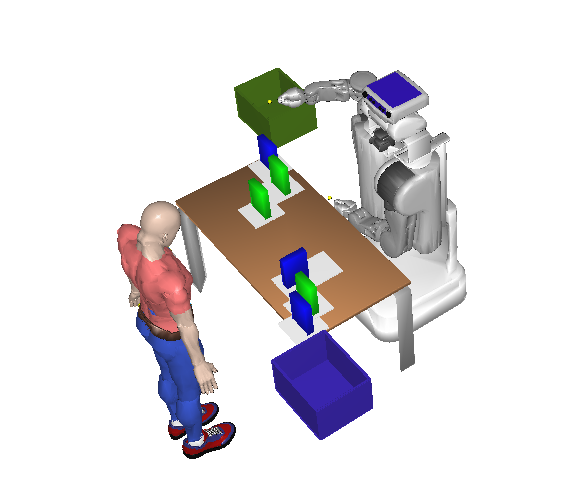
\includegraphics[width=0.3\textwidth]{figs/Chapter7/InitSecondScenario1.png}
       \label{subfig:InitSecondScenario1}
   }
    %~
	\subfigure[Another possible initial set-up. In this situation the robot thinks it can access the blue object in the middle of the table. However, the green object in front of it blocks its access.]{
        \centering
        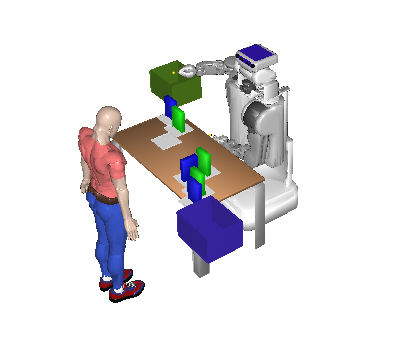
\includegraphics[width=0.3\textwidth]{figs/Chapter7/InitSecondScenario2.png}
       \label{subfig:InitSecondScenario2}
   }
    %~
	\subfigure[One possible way for the robot to access the blue object it was not able to reach is to move to another position.]{
        \centering
        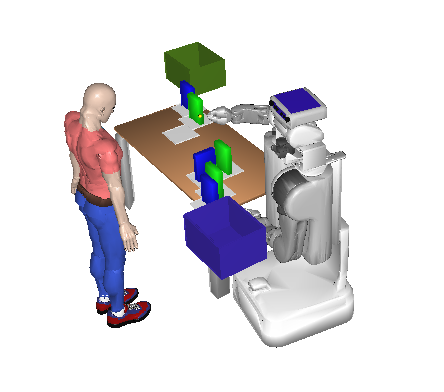
\includegraphics[width=0.3\textwidth]{figs/Chapter7/solutionSecondScenario.png}
       \label{subfig:solutionSecondScenario}
   }
    \caption{Description of the task used with the second architecture. In this task, the human and the robot have to remove all the objects of the table and put them in the box of the same color. At the beginning of the interaction several objects are accessible by the robot, others by the human and others by both agents. The green box is accessible by the robot and the blue one by the human. The placements are the white squares on the table.}
    \label{fig:firstTask}
\end{figure*}

As there are more objects and more actions to perform for the robot, the number of possible ways to achieve the task highly increases. Indeed, in the initial set-up of the previous task HATP needed around 145ms to find a plan to achieve the goal. In this new task it takes around 22s to find a plan. Consequently, the difference of cost between the MF and HATP should make more difference in this experiment.

\paragraph{Difference between planning and geometry}

In order to get closer from possible real life situation, we introduced a geometrical problem in the task. Indeed, sometimes it can happen that the knowledge computed by the robot is not accurate and that, consequently, the computed plan is not valid at execution. In our task, there are two placements in the middle of the table (accessible both by the human and the robot) which are close to each other. Each time an object is on one of these placement, the robot thinks it can reach it. when there is an object in only one of the placement (as in Fig.~\ref{subfig:InitSecondScenario1}) the robot can effectively reach the object. However, when there is an object in both placements, the robot cannot reach the one in the farthest placement as the other one blocks its access (see Fig.~\ref{subfig:InitSecondScenario2}). The Situation Assessment is not able to differentiate the two situations and in each case it will estimate that all objects in these placements are reachable by the robot. The robot will discover that it can not reach an object at motion planning time and so, the initial HATP plan will not take this into account (but when the action to pick the object not reachable failed, the robot will update its knowledge and so the new HATP plan). To access an object not reachable by it the robot can either navigate to another position (as in Fig.~\ref{subfig:solutionSecondScenario}), remove the object which blocks the access or get the object from the human (through handover).

The MF should allow the robot to learn in which case an object is really reachable by the robot and in which case another solution is preferred to get the object.

\paragraph{Different human behaviors}

Finally, in the previous task, one of the reason HATP was performing very well was that the human always executed the actions planned for him. In real life, even if the human is collaborative, he does not necessarily take the same decisions as the ones HATP took for him. In this task, we introduced three different kinds of human behavior:
\begin{itemize}
\item \textbf{The collaborative human:} it picks all objects accessible by him (with a priority for blue ones), throws the blue objects in the blue box and participates to all handover engaged by the robot.
\item \textbf{The anti-handover human:} it picks all the blue objects accessible by him, throws the blue objects in the blue box but does not participate to handover engaged by the robot (he does not react when the robot tries to execute a handover, the robot waits a few time and abort the action).
\item \textbf{The lazy human:} it picks the blue objects accessible only by him (and not the ones the robot can access), throws the blue objects in the blue box and does not participate to handover engaged by the robot.
\end{itemize}

\subsection{Results}

\begin{figure*}[!h]
\centering
	\subfigure[Mean cumulative reward for the system with only HATP. We can see that the system performs better with a collaborative human (nice), then with an human rejecting handover (noHand) and then with a lazy human (lazy).]{
        \centering
        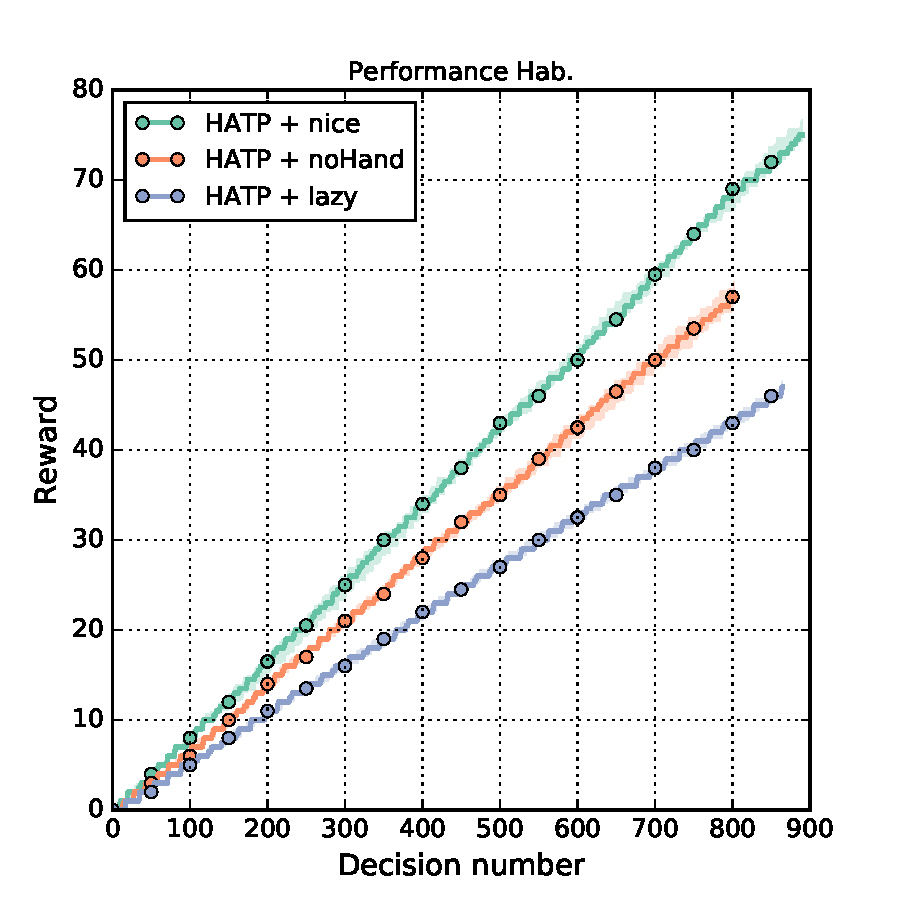
\includegraphics[width=0.45\textwidth]{figs/Chapter7/reward_HATP.pdf}
       \label{subfig:reward_HATP}
   }
    %~
	\subfigure[Mean cumulative reward for the system with only the MF. Different values for the MF parameters have been tested in order to find the best configuration in this task]{
        \centering
        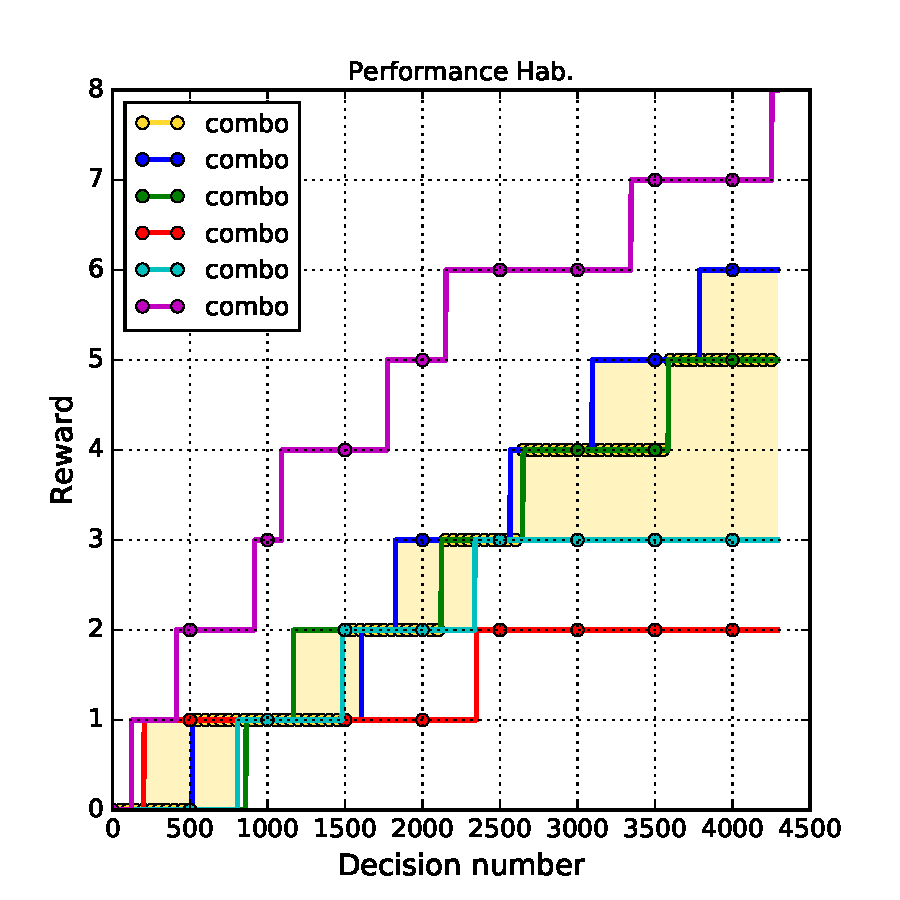
\includegraphics[width=0.45\textwidth]{figs/Chapter7/reward_MFalone.pdf}
       \label{subfig:reward_MFalone}
   }
    %~
	\subfigure[Mean cumulative reward for the system with the combination of both experts; Different values for the arbitration criteria parameters have been tested in order to find the best configuration in this task.]{
        \centering
        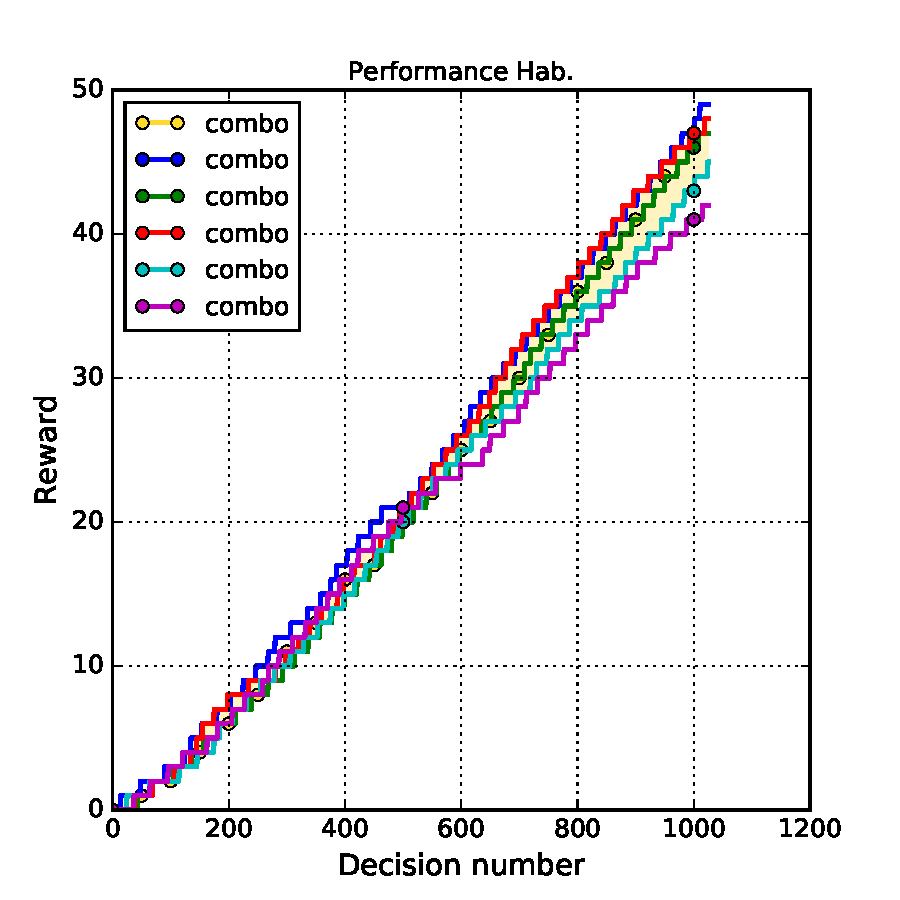
\includegraphics[width=0.45\textwidth]{figs/Chapter7/reward_combo.pdf}
       \label{subfig:reward_combo}
   }
    \caption{Mean cumulative reward for each conditions tested (HATP only, MF only and combination). The results are for 10 runs of approximatively 40 minutes in each conditions where the robot repeatedly fulfils the task.}
    \label{fig:resultsFirstTask}
\end{figure*}


We first tried the new architecture and task with HATP as the only expert. We can see in Fig.\ref{subfig:reward_HATP} that, as expected, HATP performs better with a collaborative human which will have a behavior closer than the one its planned that with humans with less collaborative behaviors. 

Then, we tested the system with the MF alone and with different parameters of the learning algorithm in order to get the better possible instantiation for this task. In a first step, we did it with a collaborative human and with only one possible initial set-up without geometrical complications. We can see in Fig.~\ref{subfig:reward_MFalone} that, as expected, the MF alone performs poorly compared to HATP.

Then, we tested the combination of both experts. In a first step, we tested it with the collaborative human and with only one possible initial set-up without geometrical complications. We tested several parametrisations of the arbitration criteria in order to get the best implementation for this task. However, we noticed that, even when we put the system in the best possible situation, it performs barely as well as HATP in its worst case (the task was solved around 45 times in each cases, see Fig.~\ref{subfig:reward_combo}). Indeed, with a more complex task, the bootstrap effect of HATP was not enough for the MF to learn a sufficiently good action policy. We tried with some runs way longer (several hours) but it was still not sufficient for the MF to learn a correct policy. 

Moreover, even if we tried to reduce computation time by putting the meta controller upstream from the experts, the effect was not the one expected. Indeed, the meta controller here is probabilist and so, even if the probability to choose the MF becomes higher than HATP, it can still happen for HATP to be chosen. In this case, a whole plan is computed by HATP even if we ask it only one action during the task. Consequently, the planning time remains the same than if HATP follows its plan alone to achieve the task.

\section{Conclusion}

In this chapter, we presented an architecture allowing to combine learning (a model free algorithm) and planing (a human-aware task planer HATP) during the robot decisional process. First results shown that HATP allows to bootstrap the learning and so to quickly learn a consistent and acceptable behavior for the robot.

In a second time, we tried to show the benefits of the learning in the system. Despite the facts that the result was not the one expected, we can still learn some lessons from this work and think of solutions to improve the system. One first possible modification would be to rework on the learning algorithm in order to study if there is method more adapted to this context. Then, another amelioration would be to look for a new arbitration criteria between the two experts. Maybe a criteria with an hysteresis in order to reduce switches between experts in a task and allow them to have time to develop their own strategy (and not having one expert breaking the strategy the other tried to set-up) would be a good idea. Finally, one interesting idea is to allow HATP to have a feedback on what is learned by the MF. Indeed, the knowledge of HATP concerning the actions is put off-line and is not updated during the interaction. For example, maybe the learning can provide the real time needed to execute an action or its probability of success given what was learned from previous interactions.


\ifdefined\included
\else
\bibliographystyle{StyleThese}
\bibliography{These}
\end{document}
\fi
